
\section{Стабилизация программных движений голономной механической системы } \label{p31}
\paragraph{}
 Рассмотрим математическую модель трехзвенного манипулятора, состоящую из трех абсолютно жестких звеньев $G_1, G_2, G_3$, представляющих собой однородные стержни. Манипулятор установлен на неподвижном основании, на которое опирается звено $G_1$. Звено $G_1$ таким образом, может совершать только вращения вокруг вертикальной оси. Звенья соединены между собой двумя идеальными цилиндрическими шарнирами $O_1$, и $O_2$ таким образом, что звенья $G_2$ и $G_3$ могут совершать движения только в вертикальной плоскости. Центр масс $C_1$ звена $G_1$ лежит на луче  $O_1 O_2$. Положение центра масс $C_2$ звена $G_2$ не совпадает с положением шарнира $O_2$. На конце звена $G_3$ находится груз, перемещаемый манипулятором.
 
 Введем обозначения: $q_i (i=1, 2, 3)$ --- углы поворотов звеньев манипулятора; $Q_i (i = 1, 2, 3)$ ---  управляющие моменты относительно осей соответствующих звеньев; $l_i$  ---  длина   $i$-го звена;   $m_i$ --- масса  $i$-го звена;    $m_0$ ---  масса перемещаемого груза;  $m_{30} = m_0 + m_3$; $J_{01}$  ---  момент инерции первого звена относительно оси вращения; $r_2$ и $r_3$ --- соответственно расстояния от центров тяжести второго и третьего звеньев с перемещаемым грузом относительно осей соответствующих звеньев; $g$ --- ускорение свободного падения.
 Уравнения движения манипулятора имеют вид:
 
 \begin{equation}
 \begin{cases}
 (J_{01} + m_2 r_2^2 \sin^2 q_2 + m_{30} (l_2 \sin q_2 + r_3 \sin q_3)^2) \ddot q_1 + \\ + 2 (m_2 r_2^2 \sin q_2 \cos q_2 + m_{30} (l_2 \sin q_2 + r_3 \sin q_3) l_2 \cos q_2) \dot q_1 \dot q_2 + \\ + 2 m_{30} (l_2 \sin q_2 + r_3 \sin q_3) r_3 \cos q_3 \dot q_1 \dot q_3 = Q_1,
 \\
 (m_2 r_2^2 + m_3 l_2^2) \ddot q_2 + \frac12 m_{30} l_2 r_3 \cos(q_2 - q_3) \ddot q_3 + \frac12 m_{30} l_2 r_3 \sin (q_2 - q_3) \dot q_3^2 - \\ - (m_{30} (l_2 \sin q_2 + r_3 \sin q_3) l_2 + m_2 r_2^2 \sin q_2) \cos q_2 \dot q_1^2 + (m_2 r_2 + m_{30} l_2) g \sin q_2 = Q_2,
 \\
 \frac12 m_{30} l_2 r_3 \cos(q_2 - q_3) \ddot q_2 + m_{30} r_3^2 \ddot q_3 - \frac12 m_{30} l_2 r_3 \sin (q_2 - q_3) \dot q_2^2 - \\ - m_{30} (l_2 \sin q_2 + r_3 \sin q_3) r_3 \cos q_3 \dot q_1^2 + m_{30} g r_3 \sin q_3 = Q_3.
 \end{cases}
 \end{equation}
 
 \begin{figure}[h]
 	\centering
 	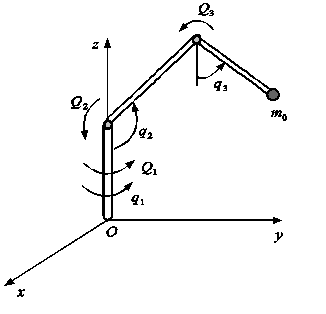
\includegraphics{3chain}
 	\caption{Модель трехзвенного манипулятора}
 	\label{fig:manip1}
 \end{figure}
 
 Пусть $q=(q_1, q_2, q_3)$ --- вектор обобщенных координат представленной выше системы. Таким образом, уравнения движения можно представить в следующей векторно-матричной форме: $A(q) \ddot q + C(q, \dot q) \dot q + K \dot q = Q$ где 
 
 \vspace{5mm}
 
 $$A(q) =
 \begin{pmatrix}
 a_{11} && 0 && 0  \\
 0  && a_{22} && a_{23} \\
 0 && a_{32} &&  a_{33}\\
 \end{pmatrix}$$
 
 \vspace{5mm}
 
 Элеменыт матрицы инерции $A(q):$
 
 $$a_{11} = J_{01} + m_2 r_2^2 \sin^2 q_2 + m_{30} (l_2 \sin q_2 + r_3 \sin q_3)^2$$
 $$a_{22} = m_2 r_2^2 + m_3 l_2^2$$
 $$a_{23} = \frac12 m_{30} l_2 r_3 \cos(q_2 - q_3)$$
 $$a_{32} = a_{23}$$
 $$a_{33} = m_{30} r_3^2$$
 
 $$C(q, \dot q)= 
 \begin{pmatrix}
 c_{11} && 0 && c_{13} \\
 c_{21} && 0 && 0 \\
 c_{31} && c_{32} && 0\\
 \end{pmatrix}$$
 
 Элементы матрицы $C(q, \dot q):$
 
 $$c_{11} = 2 (m_2 r_2^2 \sin q_2 \cos q_2 + m_{30} (l_2 \sin q_2 + r_3 \sin q_3) l_2 \cos q_2) \dot q_2$$
 $$c_{13} = 2 m_{30} (l_2 \sin q_2 + r_3 \sin q_3) r_3 \cos q_3 \dot q_3$$
 $$c_{21} = - (m_{30} (l_2 \sin q_2 + r_3 \sin q_3) l_2 + m_2 r_2^2 \sin q_2) \cos q_2 \dot q_1$$
 $$c_{31} = - m_{30} (l_2 \sin q_2 + r_3 \sin q_3) r_3 \cos q_3 \dot q_1$$
 $$c_{32} = - \frac12 m_{30} l_2 r_3 \sin (q_2 - q_3) \dot q_2$$
 
 \vspace{5mm}
 
 $A(q)$ --- положительно определенная матрица инерции системы.
 
 \section{Построение управления}%
 \markright{\thechapter.\thesection.\hspace{1em}Построение управления}{}
 \label{sec2.3}
 Пусть  $q = (q_1, q_2, q_3)^{'}$ --- вектор обобщенных координат рассматриваемой механической системы и $X = {q^0(t):[t_0, + \infty) \to R^3, \| q^0(t) \| \le q_0, \| \dot q^0 \| \le g_1,\| q^0(t) \| \le q_0, \| \ddot q^0 \| \le g_2}$ есть заданное множество программных движений манипулятора в виде ограниченных дважды непрерывно дифференцируемых функций $q = q^0(t)$ с ограниченными производными при $t \in [t_0, + \infty)$.  Символом   $\| \cdot \|$ обозначена евклидова норма вектора. Уравнения движения (3.1) можно представить в следующей векторно-матричной форме: 
 
 \begin{equation}
 A(q) \ddot q + C(q, \dot q) \dot q + K \dot q = Q,     
 \end{equation}

 где $A(q)$ --- положительно определенная матрица инерции системы, $C(q, \dot q) = \sum_{i = 1}^{3} \dot q_i C_{(i)} (q),$ , $j,k$-ый элемент $c_{(i)jk} (q)$ матрицы $C_{(i)}(q)$  определяется в виде $c_{(i)jk} (q) = \frac12 (\frac{\partial a_{ij}}{\partial q_k} + \frac{\partial a_{ij}}{\partial q_i} - \frac{\partial a_{ij}}{\partial q_j} )$;
 $K$ --- матрица коэффициентов моментов сил вязкого трения, действующих в системе.
 Система (3.2) имеет следующее свойство: матрица $\dot A(q(t)) - 2 C(q(t), \dot q(t))$  является  кососимметричной.
 Пусть $q^0(t) \in X$ --- какое-либо программное движение системы (3.2), реализуемое программным управлением $Q = Q^{(0)}(t)$, т.е. имеет место тождество $A(q^0(t)) \ddot q^0(t) + C(q^0(t), \dot q^0(t)) \dot q^0(t) + K \dot q^0(t) \equiv Q^{(0)}(t)$.
 Введем возмущения $x = q - q^0(t)$ и составим уравнения возмущенного движения в векторно-матричном виде:
 \begin{equation}
 A^{(1)}(t, x) \ddot x + C^{(1)}(t, x, \dot x) \dot x + K \dot x = Q^{(1)}(t, x, \dot x) + Q^{(2)}(t, x, \dot x),
 \end{equation} 
 где $A^{(1)}(t, x) = A(x + q^0(t))$, $C^{(1)}(t, x, \dot x) = C(x + q^0(t)$, $\dot x + \dot q^0(t))$, $Q^{(1)}(t, x, \dot x) = Q - Q^{(0)}(t)$, $Q^{(2)}(t, x, \dot x) = (A^{(1)}(t, 0) - A^{(1)}(t, x)) \ddot q^0(t) + (C^{(1)}(t, 0, 0) - C^{(1)}(t, x, \dot x)) \dot q^0(t)$.
 Рассмотрим задачу построения управляющего воздействия $Q^{(1)}(t, x, \dot x)$, при котором невозмущенное движение $\dot x = x = 0$ системы (3.3) было бы равномерно асимптотически устойчиво, или, иначе, управление $Q = Q^{(1)}(t, q-q^{(0)}(t), \dot q - \dot q^{(0)}) + Q^{(0)}(t)$ обеспечивало бы стабилизацию программного движения   системы (3.2).
 
  \section{Синтез управления в задаче стабилизации программного движения манипулятора}% 
 Рассмотрим решение задачи стабилизации в области $G = {(x, \dot x) \in R^6 : \|x\| < \epsilon, \|\dot x \| < \epsilon, \epsilon = const>0}$
 с помощью непрерывного управления вида
 
 \begin{equation*}
  Q^{(1)} (x, \dot ) = B(\dot x + p(x)),
 \end{equation*}
 
 где $B \in R^{3 \times 3}$ есть матрица коэффициентов усиления сигналов, подлежащая определению; $p(x)$ --- непрерывно дифференцируемая вектор-функция, такая, что $\| p(x) \| \ge p_0(x) > 0, p_0(0) = 0$.
 Возьмем для системы (3.3) вектор-функцию Ляпунова $V = (V^1, V^2)^{'}$ с коэффициентами вида $V^1 = \|p(x)\|, V^2 = \sqrt{(\dot x + p(x))^{'} A^{(1)} (t, x) (\dot x + p(x))}$.
 
 Вычисляя производные по времени от квадратов компонент вектор-функции Ляпунова  в силу системы (3.3), получим 
 \begin{equation*}
 \frac{d}{dt} (V^1(x))^2 = 2 V^1 \dot V^1 = 2 p^{'} \dot p = 2 p^{'} \frac{\partial p }{\partial x} \dot x = -2 p^{'} \frac{\partial p }{\partial x} p + 2 p^{'} \frac{\partial p }{\partial x}(\dot x + p),
 \end{equation*}
 
 \begin{equation*}
  \frac{d}{dt} (V^2(x))^2 = 2 V^2 \dot V^2 = 2(\ddot x + \dot p)^{'} A^{(1)} (\dot x + p) + (\dot x + p)^{'} \dot A^{(1)} (\dot x + p) = 2(- C^{(1)}(t, x, \dot x) \dot x - R \dot x + Q^{(1)}(x, \dot x) + Q^{(2)}(t, x, \dot x))^{'} (\dot x + p) + 2 \dot p^{'} A^{(1)} (\dot x + p) + (\dot x + p)^{'} \dot A^{(1)} (\dot x + p).
 \end{equation*}
 
 Отсюда получим следующие оценки:
 $\dot V^1 \le - \mu_1 V^1 + \frac{m_1}{\lambda(t, x)} V^2, \dot V^2 \le \frac{m_2}{\lambda(t, x)} V^1 - \frac{\mu_2}{\lambda^2(t,x)}$,
 где положительные постоянные $\mu_2, \mu_2, m_1, m_2$  и функция $\lambda(t,x)$  определяются из следующих условий:
 \begin{equation}
 p^{'} \frac{\partial p}{\partial x} p \ge \mu_1 \|p\|^2, \|\frac{\partial p}{\partial x}\| \le m_1, \lambda(t, x) \| \dot x + p \| = V^2,
 \end{equation}
 
 \begin{equation}
 \| Q^{(2)} (t, x, \dot x) \le (m_2 - \| C^{(1)}(t, x, \dot x) + K - A^{(1)}(t, x) \frac{\partial p}{\partial x}\|) \|p\|
 \end{equation}

\begin{equation}
 \lambda_{max} (B + B^{'} - K - K^{'} + A^{(1)}(t, x) \frac{\partial p}{\partial x} + (\frac{\partial p}{\partial x})^{'} A^{(1)}(t, x)) \le -2 \mu_2
\end{equation}
 
 Здесь $\lambda_max()$ есть максимальное собственное значение соответствующей матрицы. 
 Тогда для системы (3.3) можно построить следующую систему сравнения:
 
 \begin{equation}
 \dot u^1 = - \mu_1 u^1 + \frac{m_1}{\lambda(t,x)} u^2, \dot u^2 = \frac{m_2}{\lambda(t, x)} u^1 - \frac{\mu_2}{\lambda^2(t, x)} u^2. 
 \end{equation}
 
 Согласно теореме сравнения об экспоненциальной устойчивости [5] из свойства экспоненциальной устойчивости нулевого решения системы сравнения (3.5) следует аналогичное свойство нулевого решения системы (3.3).  Можно показать, что нулевое решение системы сравнения (3.5) будет экспоненциально устойчиво при следующем условии
 $4 \mu_1 \mu_2 > (m_1 / k + m_2 k)^2, k = const>0$.
 Численное моделирование движения манипулятора при действии управления (3.4) проводилось при следующих значениях параметров манипулятора и программной траектории
 
\begin{equation*}
 m_2=15 \text{ кг}, m_3=2,5 \text{ кг}, m_0 = 2 \text{ кг}, l_2 = 1 \text{ м}, r_2=0,5 \text{ м}, r_3 = 0,5 \text{ м}, J_{01} = 0,1 \text{ кг} \cdot \text{м\textsuperscript{2}}, q_1^0(t) = 0,2t, q_2^0(t) = 1,5 + 0,5 sin t, q_3^0(t) = 0,5 sin(0,5 t).
\end{equation*}
 
 На рисунках 2–4 представлены результаты моделирования. Пунктирной линией обозначены  составляющие программного движения, а сплошной – реального движения системы.